
\section{Sistemi interconnessi - esteso}
È possibile suddividere un sistema comunque complesso, composto da più
sottosistemi che interagiscono tra loro.
Al fine di formalizzare correttamente i sistema interconnessi si presentano i
tre blocchi principali.

Il primo è il blocco sistema, rappresenta il modello di un sistema, disegnato
mediante un rettangolo, con le frecce in ingresso e in uscita si indicano le
variabili di ingresso e uscita.
$$
Y_f(s) = W(s)U(s)
$$
\begin{figure}[h]
\centering
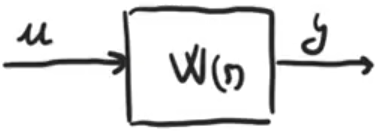
\includegraphics[width=0.3\linewidth]{blocco_sistema}
\end{figure}

Il secondo elemento è il nodo diramatore, ha un ingresso, poi con un punto
calcato si suddividono le uscite (nel dominio del tempo o di Laplace
$$
y_1(t) = y_2(t) = y_3(t) = u(t)
$$
\begin{figure}[h]
\centering
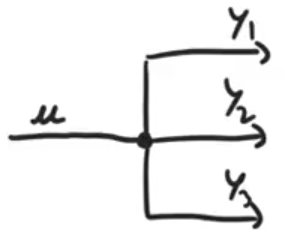
\includegraphics[width=0.3\linewidth]{blocco_nodo}
\end{figure}

\newpage
Il nodo sommatore invece, rappresentato mediante un cerchio o un quadrato
esegue somme o sottrazioni degli ingressi, fornendo una sola uscita
$$
y(t) = u_1(t) - u_2(t) + u_3(t)
$$
\begin{figure}[h]
 \centering
 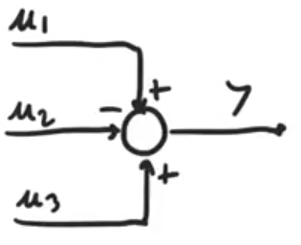
\includegraphics[width=0.3\linewidth]{blocco_sommatore}
\end{figure}

Per ottenere la rappresentazione di tutto il sistema è comodo operarne la sua
riduzione, per via algebrica o più comodamente per via grafica.
Le regole di riduzione si basano sulla presenza di tre connessioni canoniche,
in serie, in parallelo e in retroazione.

\subsection{Connessione in serie}
Due o più blocchi sono connessi in serie se l'ingresso del blocco
successivo coincide con l'uscita del precedente.
\begin{figure}[h]
\centering
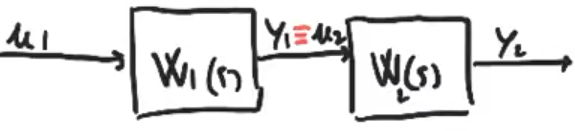
\includegraphics[width=\picwid]{blocchi_serie}
\end{figure}
Dal punto di vista sistemistico la serie può essere vista come un unico blocco
più grande con un'unica funzione di trasferimento $W(s)$ con ingresso $u$ e
uscita $y$.

Si ricava la riduzione, si presentano le relazioni algebriche dei due blocchi e
il vincolo topologico
$$\left\{\begin{aligned}
Y_1(s) &= W_1(s)U_1(s) \\
Y_2(s) &= W_2(s) U_2(s) \\
Y_1(s) &= U_2(s)
\end{aligned}\right.
\quad
\begin{aligned}
Y(s) &= Y_2(s) = W_2(s)U_2(s) = W_2(s)Y_1(s) =\\
&=W_2(s)W_1(s)U_1(s) = W_2(s)W_1(s)U(s)
\end{aligned}$$
La funzione di trasferimento del blocco ridotto è dunque pari al prodotto delle
due funzioni di trasferimento dei sottosistemi.
Se il sistema è SISO la moltiplicazione è commutativa, non è vero per i sistemi
non SISO.

\newpage
\subsection{Connessione in parallelo}
Due o più sottosistemi sono connessi in parallelo se condividono lo stesso
ingresso, uscita di un nodo diramatore, e la loro uscita viene combinata in un
nodo sommatore.
\begin{figure}[h]
\centering
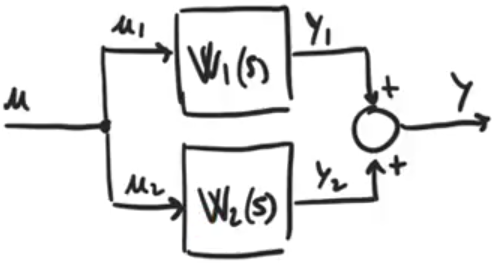
\includegraphics[width=\picwid]{blocchi_parallelo}
\end{figure}

